\section{Introduction}

The `design' of GLIMMER is a consequence of the way it has been
developed. Initially, as a stand-alone model with a single domain, module
variables were used to hold all model fields and parameters. With the move to
use GLIMMER as the ice model component within GENIE, and the desire to enable
several active regions to be run simultaneously, the module variables were
converted into components of derived types, and an extra layer added on top of
the exisiting structure to deal with global fields and parameters, and deal
with the downscaling/interpolation of input fields. The result is a structure
that is probably more complex than it needs to be, but still hopefully
reasonably logical.


\section{Physics documentation}

\subsection{Ice temperature evolution routines}

\subsubsection{Summary}
Call structure (filenames in brackets).
\begin{itemize}
    \item subroutine testinisthk [glimmer\_setup] and
    \item subroutine glimmer\_i\_tstep [glimmer\_object] call
    \item subroutine timeevoltemp [glimmer\_temp] calls
    \item subroutine calcartm [glimmer\_temp] and
    \item subroutine timeders [glimmer\_thck] and
    \item subroutine gridwvel [glimmer\_velo] and
    \item subroutine wvelintg [glimmer\_velo] and
    \item subroutine chckwvel [glimmer\_velo] and
    \item subroutine finddisp [glimmer\_temp] and
    \item subroutine hadvall [glimmer\_temp] and
    \item subroutine hadvpnt [glimmer\_temp] and
    \item subroutine findvtri [glimmer\_temp] and
    \item subroutine tridag [glimmer\_temp] and
    \item subroutine corrpmpt [glimmer\_temp] and
    \item subroutine swapbndt [glimmer\_temp] and
    \item subroutine calcbmlt [glimmer\_temp] and
    \item subroutine calcflwa [glimmer\_temp]
\end{itemize}

\noindent Modules used.
\begin{itemize}
    \item
\end{itemize}

\subsubsection{Introduction}
The section describes the routines that are concerned with
calculating the three-dimensional distribution of temperature
within the ice mass.  They can be broken down into five groups.
\begin{itemize}
    \item determining air temperature (upper boundary
    condition) [\texttt{calcartm}];
    \item determining vertical velocity field from existing
    horizontal velocity fields (normally only needed if temperature is being calculated) [\texttt{wvelintg}, chckwvel];
    \item routines associated with vertical grid coordinate
    system [\texttt{gridwvel}, \texttt{timeders}];
    \item the main temperature solver [\texttt{finddisp, hadvall, hadvpnt, findvtri, tridag, corrpmpt, swapbndt}];
    \item ancillary calculations that only make sense if temperature is being calculated
    [\texttt{calcbmlt}, \texttt{calcflwa}].
\end{itemize}

The basic quantity returned is a three-dimensional grid of
temperature in $\circ^{-1}$C (uncorrected for variations in
pressure melting point and unscaled).  Temperature is held in the
array \texttt{temp} and will be referred to here using the symbol
$T$.

In addition to temperature a number of other quantities are
calculated by these routines.  They include: basal melt rate ($m$
\texttt{bmlt} m yr$^{-1}$ scaled using \texttt{thk0/tim0}); basal
water depth ($W$ \texttt{bwat} m scaled using \texttt{thk0});
vertical velocity ($w$ \texttt{wvel} m yr$^{-1}$ scaled using
\texttt{thk0/tim0}); vertical velocity of numerical grid ($w_0$
\texttt{wgrd} m yr$^{-1}$ scaled using \texttt{thk0/tim0}); Glen's
A ($A$ \texttt{flwa} Pa$^{-3}$ yr$^{-1}$ scaled using
\texttt{vis0}); air temperature ($T_a$ $\circ^{-1}$C unscaled).
All scales are held in the module \texttt{paramets} in
\textbf{\texttt{glimmer\_paramets}}.

Three options are currently available for calculating $T$. The
particular option chosen is controlled by the input parameter
\texttt{whichtemp} (\texttt{gln} file).

\begin{description}
    \item[0] Set whole column to the appropriate surface air temperature ($T_a$).
    \item[1] This option is the main solver that determines temperature
    at the new time step from the appropriate three-dimensional
    advection-diffusion equation.
    \item[2] Set the upper surface temperature to $T_a$ and do a linear
    interpolation from this value to 0 $^\circ$C at the lower
    surface. Check for pressure melting and adjust any
    temperatures that are above melting point.
\end{description}

The subroutine \texttt{timeevoltemp} controls calculation of the
$T$ etc. It is called in the main time loop in
\textbf{\texttt{glimmer\_object}} and resides in
\textbf{\texttt{glimmer\_temp}}.

\section{Data structure}

The derived type \texttt{glimmer\_params} is the top-level data-structure in
GLIMMER. It contains the global parameters for the model, as well as the
global fields used in the temporal averaging of input fields. Its primary
function, however, is to hold an array of ice model instances (type
\texttt{glimmer\_instance}). This array is allocated at run-time. Each ice
model instance contains instances of derived types (\texttt{projection} and
\texttt{downscale}) concerning the relationship between the local and global
model grids, as well as upscaling parameters (which should have their own
derived type, really), and an instance of \texttt{glimmer\_global\_type}. This
last derived type contains single instances of eighteen other derived types,
which were replacements for the variable-containing modules of the original
ice model. It is debatable whether \texttt{glimmer\_global\_type} is strictly necessary,
and it might be worth reorganising the whole structure at some point, though
this would obviously be a big job. The situation is summarised in figure
\ref{main_class_diagram}.

\begin{figure}
\centering
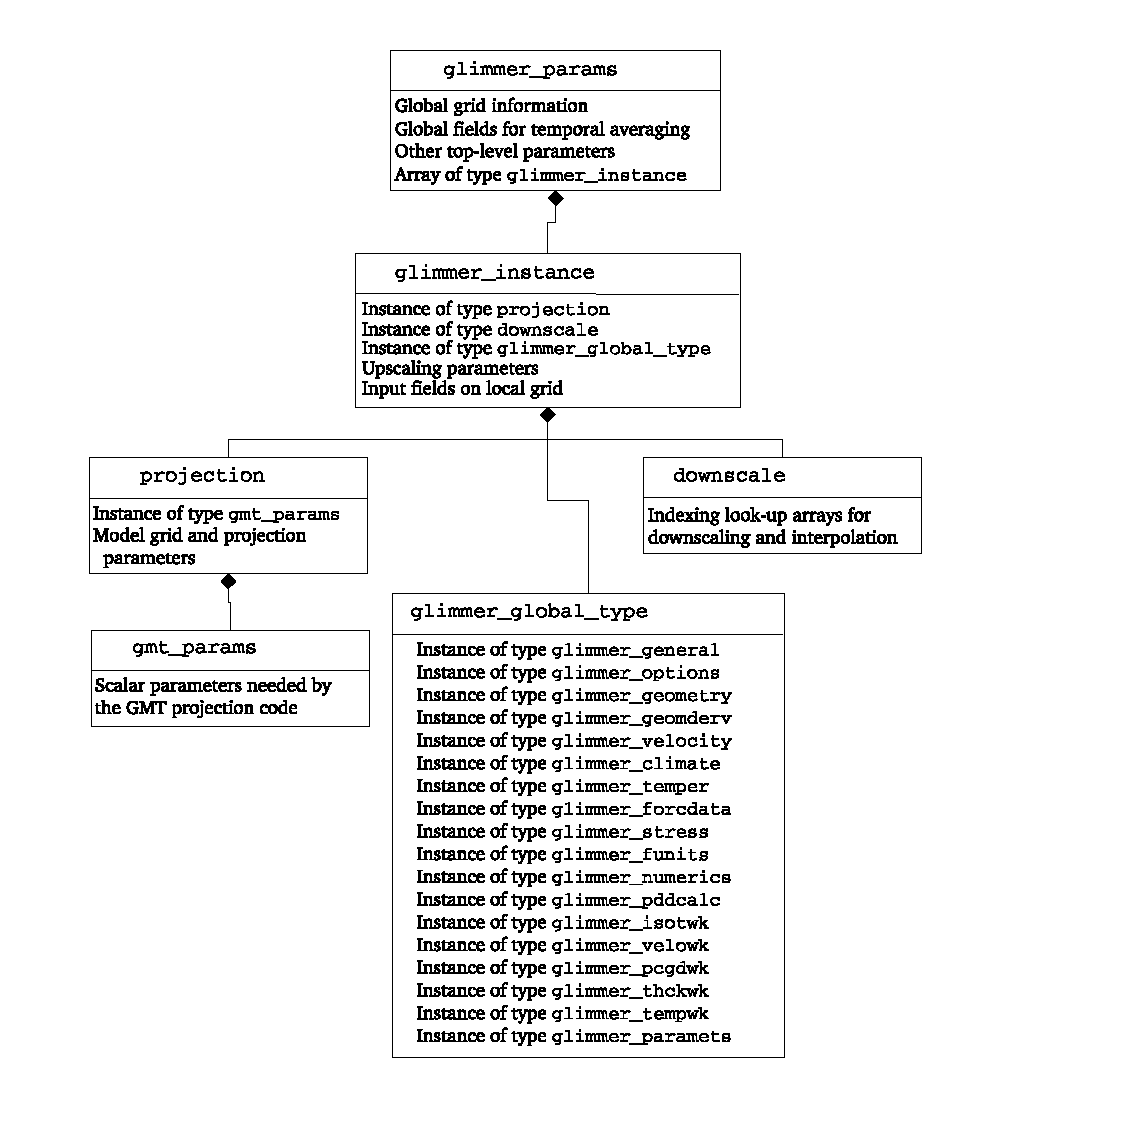
\includegraphics[width=\textwidth]{\dir/figures/class_diagram.eps}
\caption{Main `Class Diagram' for GLIMMER. The relationship between the top-level
  \texttt{glimmer\_params} type and its component types is shown. The
  components of the \texttt{glimmer\_global\_type} type are formed from the
  modules of the original ice model.}
\label{main_class_diagram}
\end{figure}

\section{Configuration File Parser}\label{dg.sec.config_file}
The run--time behaviour of the ice sheet model is controlled by configuration files. The old file format is based on Fortran namelists. The new configuration file format is loosely based on the format of Windows \texttt{.ini} files with sections containing name/value pairs. The new format is more flexible and can be easily understood by reading the configuration files. This section contains a description of the configuration file parser API.

\subsection{File Format}
The parser assumes a maximum number of 250 characters per line. Leading and trailing white space is ignored. Names are case sensitive.
\begin{description}
\item[Comments:] Empty lines and lines starting with \texttt{!}, \texttt{;} or \texttt{\#} are ignored.
\item[Sections:] Section names are enclosed with square prackets, \texttt{[]} and can be 20 character long.
\item[Parameters:] Parameter names are separated from their associated values with either \texttt{:} or \texttt{=}. The names can be 20 characters long. Values can be 200 characters long.
\end{description}

An example configuration file:
\begin{verbatim}
;a comment
[a section]
an_int  : 1
a_float = 2.0
a_char  = hey, this is rather cool
an_array = 10. 20. -10. 40. 100.

[another section]
! more comments
foo : bar
\end{verbatim}

\subsection{Architecture Overview}
The configuration data is stored as linked list. Each section is described by the following list element:
\begin{verbatim}
  type ConfigSection
     character(len=namelen) :: name
     type(ConfigValue), pointer :: values=>NULL()
     type(ConfigSection), pointer :: next=>NULL()
  end type ConfigSection
\end{verbatim}
The parameter name/value pairs defined in each section are stored in another linked list:
\begin{verbatim}
  type ConfigValue
     character(len=namelen) :: name
     character(len=valuelen) :: value
     type(ConfigValue), pointer :: next=>NULL()
  end type ConfigValue
\end{verbatim}
These linked lists are setup and read using subroutines.

\subsection{API}
\begin{description}
\item[Reading configuration files] Configuration files are read using \texttt{ConfigRead}. This subroutine parses the configuration file and populates the linked lists.
\begin{verbatim}
subroutine ConfigRead(fname,config)
  character(len=*), intent(in) :: fname
  type(ConfigSection), pointer :: config
end subroutine ConfigRead
\end{verbatim}
The pointer \texttt{config} contains the first section of the configuration file.
\item[Dumping configuration] The subroutine \texttt{PrintConfig} traverses the linked lists and prints them to standard output.
\begin{verbatim}
subroutine PrintConfig(config)
  type(ConfigSection), pointer :: config
end subroutine PrintConfig(config)
\end{verbatim}
\item[Searching for a Section] The subroutine \texttt{GetSection} can be used to find a specific section.
\begin{verbatim}
subroutine GetSection(config,found,name)
  type(ConfigSection), pointer :: config
  type(ConfigSection), pointer :: found
  character(len=*),intent(in) :: name
end subroutine GetSection
\end{verbatim}
On exit the pointer \texttt{found} will point to the first section called \texttt{name}. \texttt{found} points to \texttt{NULL()} if the section \texttt{name} is not found.
\item[Reading parameters] Paramter name/value pairs are found using the \texttt{GetValue} family of subroutines. \texttt{GetValue} provides an interface to the individual subroutines \texttt{GetValueChar}, \texttt{GetValueInt}, \texttt{GetValueReal}, \texttt{GetValueIntArray} and \texttt{GetValueRealArray}.
\begin{verbatim}
subroutine GetValue(section,name,val)
  type(ConfigSection), pointer :: section
  character(len=*),intent(in) :: name
  sometype :: val
  integer,intent(in), optional :: numval
end subroutine GetValue
\end{verbatim}
\texttt{section} is the section that should be searched for the parameter \texttt{name}. On exit \texttt{val} contains the parameter value if it is found, otherwise it is unchanged. 

The array versions of \texttt{GetValue} expect value to be a pointer to a one--dimensional array. \texttt{val} is deallocated if it was allocated on entry. The array versions of \texttt{GetValue} also accept an optional value, \texttt{numval}, with which the maximum number of array elements can be set. The default is 100. Array elements are separated by white space.
\end{description}

\section{netCDF I/O}
The netCDF\footnote{\texttt{http://www.unidata.ucar.edu/packages/netcdf/}} library is used for platform independent, binary file I/O. GLIMMER makes use of the f90 netCDF interface. The majority of the source files are automatically generated from template files and a variable definition file using a python script. The netCDF files adhere to the CF\footnote{\texttt{http://www.cgd.ucar.edu/cms/eaton/cf-metadata/index.html}} convention for naming climatic variables. The netCDF files also store parameters used to define the geographic projection.

The netCDF related functionality is split up so that other subsystems of the model can easily define their own variable sets without the need to recompile the main model. These subsystems can also define their own dimensions and access the dimensions defined by other subsystems. The only restriction is that names should not clash. Have a look at the implementation of the \texttt{eis} climate driver.
\subsection{Data Structures}
Information associated with each dataset is stored in the \texttt{glimmer\_nc\_stat} type. Variable and dimension ids are retrived from the data set by using the relevant netCDF library calls. Meta data (such as title, institution and comments) is stored in the derived type \texttt{glimmer\_nc\_meta}.

Input and output files are managed by two separate linked lists. Elements of the input file list contain the number of available time slices and information describing which time slice(s) should be read. Output file elements describe how often data should be written and the current time.

\subsection{The Code Generator}
Much of the code needed to do netCDF I/O is very repetative and can therefore be automatically generated. The code generator, \texttt{generate\_ncvars.py}, is written in python and produces source files from a template \texttt{ncdf\_template.in} and the variable definition file, see Section \ref{dg.sec.vdf}. The templates are valid source files, all the generator does is replace special comments with the code generated from the variable file. For further information check the documentation of \texttt{generate\_ncvars.py}\footnote{run \texttt{pydoc generate\_ncvars.py}}.

\subsection{Variable Definition File}\label{dg.sec.vdf}
All netCDF variables are defined in control files, \texttt{MOD\_vars.def}, where \texttt{MOD} is the name of the model subsystem. Variables can be modified/added by editing these files. The file is read using the python \texttt{ConfigParser} module. The format of the file is similar to Windows \texttt{.ini} files, lines beginning with \texttt{\#} or \texttt{;} or empty lines are ignored. These files must have a definition section \texttt{[VARSET]} (see Table \ref{dg.tab.vdef}).A new variable definition block starts with the variable name in square brackets []. Variables are further specified by parameter name/value pairs which are separated by \texttt{:} or \texttt{=}. Parameter names and their meanings are summarised in Table \ref{dg.tab.vdf}. All parameter names not recognised by the code generator (i.e. not in Table \ref{dg.tab.vdf}) are added as variable attributes.

\begin{table}[htbp]
  \centering
  \begin{tabular}{|l|p{10cm}|}
    \hline
    name & description \\
    \hline
    \hline
    \texttt{name} & Name of the model subsystem, e.g. \texttt{glide}. The f90 file is renamed based on this name. The f90 module and module procedures are prefixed with this name.\\
    \hline
    \texttt{datatype} & The name of the f90 type on which the netCDF variables depend.\\
    \hline
    \texttt{datamod} & The name of f90 module in which the f90 type, \texttt{datatype}, is defined.\\
    \hline
  \end{tabular}
  \caption{Each variable definition file must have a section, called \texttt{[VARSET]}, containing the parameters described above.}
  \label{dg.tab.vdef}
\end{table}

\begin{table}[htbp]
 \begin{center}
  \begin{tabular}{|l|p{10cm}|}
    \hline
    name & description \\
    \hline
    \hline
    \texttt{dimensions} & List of comma separated dimension names of the variable. C notation is used here, i.e. the slowest varying dimension is listed first.\\
    \hline
    \texttt{data} & The variable to be stored/loaded. The f90 variable is assumed to have one dimension smaller than the netCDF variable, i.e. f90 variables are always snapshots of the present state of the model. Variables which do not depend on time are not handled automatically. Typically, these variables are filled when the netCDF file is created.\\
    \hline
    \texttt{factor} & Variables are multiplied with this factor on output and divided by this factor on input. Default: 1.\\
    \hline
    \texttt{load} & Set to 1 if the variable can be loaded from file. Default: 0.\\
    \hline
    \texttt{units} & UDUNITS compatible unit string describing the variable units.\\
    \hline
    \texttt{long\_name} & A more descriptive name of the variable.\\
    \hline
    \texttt{standard\_name} & The corresponding standard name defined by the CF standard.\\
    \hline
  \end{tabular}
  \caption{List of accepted variable definition parameters.}
  \label{dg.tab.vdf}
 \end{center}
\end{table}

